\documentclass[11pt]{article}
\usepackage{amsmath, amssymb}
\usepackage{hyperref}
\usepackage{graphicx}
\usepackage{tikz}

% Define \problemname and \illustration if not using Kattis template
\newcommand{\problemname}[1]{\section*{#1}}
\newcommand{\illustration}[3]{%
    \begin{figure}[h]
        \centering
        \includegraphics[width=#1\textwidth]{#2}
        \caption{#3}
    \end{figure}
}

\begin{document}

\problemname{The Evil Word}

You are writing an essay for a notoriously strict professor who believes that certain \emph{words} carry
``evil energy.'' The professor measures the \emph{evilness} of a word by summing the ASCII values of all
characters it contains. A word with a larger total ASCII score is considered more evil.

Formally, for a word $\text{w}$ with characters $\text{w}[1], \dots, \text{w}[|\text{w}|]$, its evilness is
\[
    E(\text{w}) \;=\; \sum_{i=1}^{|\text{w}|} \text{ASCII}(\text{w}[i]).
\]

The professor's old text-processing machine does not store the full essay. Instead, it receives the input
\emph{\textbf{one word at a time}}, each word arriving as a stream of characters on a single line. As soon as
a word has been fully read, the machine computes its evilness $E(\text{w})$ and then immediately discards the
characters themselves, keeping only a small number of candidate evilness values in memory.

After each new word is processed, the professor wants to know \emph{both}:
\begin{itemize}
    \item the current \textbf{$k$-th least evil word}, and
    \item the current \textbf{$k$-th most evil word},
\end{itemize}
among all words seen so far, according to their evilness scores.

These rankings are computed over the \textbf{multiset of evilness scores}, counting duplicates.
If multiple words share the same score, ties are broken by arrival order: a word that appears \emph{later} in the input is considered more evil than an earlier word with the same score. This makes each query's answer unique.

If fewer than $k$ words have appeared so far, the professor is not satisfied with either query and expects
you to output ``-'' in its place.

\begin{figure}[htbp]
\centering
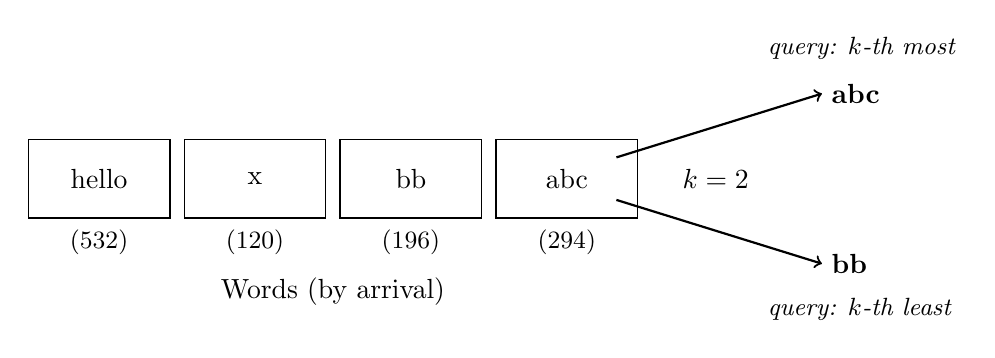
\begin{tikzpicture}[scale=0.9]

% Words in boxes
\node[draw, minimum width=1.8cm, minimum height=1cm] (hello) at (0,0) {hello};
\node at (0,-0.9) {\small (532)};

\node[draw, minimum width=1.8cm, minimum height=1cm] (xword) at (2.2,0) {x};
\node at (2.2,-0.9) {\small (120)};

\node[draw, minimum width=1.8cm, minimum height=1cm] (bb) at (4.4,0) {bb};
\node at (4.4,-0.9) {\small (196)};

\node[draw, minimum width=1.8cm, minimum height=1cm] (abc) at (6.6,0) {abc};
\node at (6.6,-0.9) {\small (294)};

\node at (3.3,-1.6) {Words (by arrival)};

% Arrows
\draw[->, thick] (7.3,0.3) -- (10.2,1.2);
\draw[->, thick] (7.3,-0.3) -- (10.2,-1.2);

% Shift the query labels ONLY
\node[anchor=south west] at (9.3,1.55) {\small\textit{query: $k$-th most}};
\node[anchor=north west] at (9.3,-1.55) {\small\textit{query: $k$-th least}};

% Answers stay in place
\node[anchor=west] at (10.2,1.2) {\textbf{abc}};
\node[anchor=west] at (10.2,-1.2) {\textbf{bb}};

% k label
\node at (8.7,0) {$k = 2$};

\end{tikzpicture}

\caption{Example with $k = 2$: the 2nd least evil word is \texttt{bb}, and the 2nd most evil word is \texttt{abc}.}
\end{figure}



\section*{Input}

The input begins with a single line containing two integers $n$ and $k$, where
\[
    1 \le k \le n \le 200\,000.
\]

The next $n$ lines each contain exactly one word, consisting only of printable ASCII characters
(codes 33 to 126, from \texttt{!} to \texttt{\~}).  
Each line provides the complete stream of characters for that word.

\section*{Output}

Output exactly $n$ lines.

After processing the $i$-th word, print two space-separated tokens describing the current
\emph{$k$-th least evil} and \emph{$k$-th most evil} words among all words seen so far (using the tie-breaking rule above):
\begin{itemize}
    \item If fewer than $k$ words have been processed, print \texttt{- -}.
    \item Otherwise, print \texttt{$L$ $R$}, where \texttt{$L$} is any word whose evilness is the $k$-th smallest
          among all scores seen so far, and \texttt{$R$} is any word whose evilness is the $k$-th largest.
\end{itemize}

If several words share the same evilness score, any valid choice for \texttt{L} or \texttt{R} will be accepted.

\section*{Sample Input/Output}

\noindent
\begin{tabular}{|p{0.45\textwidth}|p{0.45\textwidth}|}
\hline
\textbf{Sample Input 1} & \textbf{Sample Output 1} \\
\hline
\ttfamily
5\ 2\newline
hello\newline
x\newline
bb\newline
abc\newline
wow
&
\ttfamily
- -\newline
hello\ x\newline
bb\ bb\newline
bb\ abc\newline
bb\ wow
\\
\hline
\end{tabular}

\vspace{1.5em}

\noindent
\begin{tabular}{|p{0.45\textwidth}|p{0.45\textwidth}|}
\hline
\textbf{Sample Input 2} & \textbf{Sample Output 2} \\
\hline
\ttfamily
3\ 1\newline
abc\newline
xyz\newline
a
&
\ttfamily
abc\ abc\newline
abc\ xyz\newline
a\ xyz
\\
\hline
\end{tabular}

\end{document}
